\usetikzlibrary{calc}
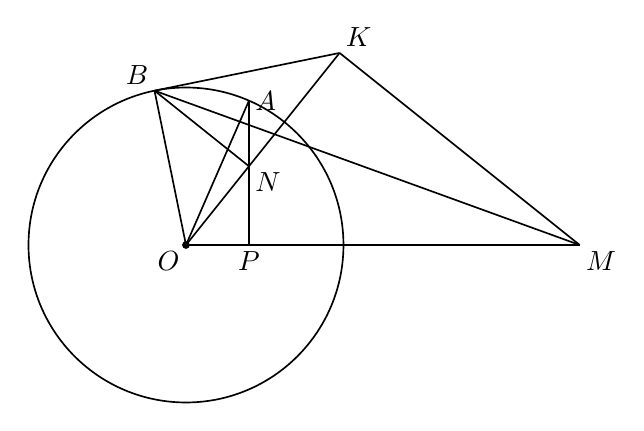
\begin{tikzpicture}[x=1cm,y=1cm,line width=.6pt,font=\normalsize]
\coordinate (O) at (0,0);
\coordinate (M) at (5,0);
\coordinate (P) at (0.8,0);
\coordinate (N) at (0.8,1.0);
\coordinate (A) at (0.8,1.833);
\coordinate (B) at (-0.3996,1.9597);
\coordinate (K) at (1.9512,2.439);
\draw (O) circle[radius=2cm];
\draw (O)--(M);
\draw (A)--(P);
\draw (O)--(B);
\draw (O)--(A);
\draw (N)--(B);
\draw (B)--(M);
\draw (O)--(K);
\draw (B)--(K);
\draw (K)--(M);
\node[below left=2pt,inner sep=0pt] at (O) {$O$};
\node[below=2pt,inner sep=0pt] at (P) {$P$};
\node[below right=2pt,inner sep=0pt] at (N) {$N$};
\node[right=2pt,inner sep=0pt] at (A) {$A$};
\node[above left=2pt,inner sep=0pt] at (B) {$B$};
\node[above right=2pt,inner sep=0pt] at (K) {$K$};
\node[below right=2pt,inner sep=0pt] at (M) {$M$};

% Explicit named circle-center points, painted after all region fills.
\fill (O) circle[radius=1.4pt];
\end{tikzpicture}
